\newpage

\section{Word Embeddings}

\epigraph{
    Nets are for fish; once you get the fish you can forget the net.\\
    Words are for meaning; once you get the meaning you can forget the words.
}{Zhuangzi}
\newpage

\subsection{Dalla semantica alla rappresentazione vettoriale}
\label{sec:semantics_to_vectors}

Questo capitolo introduce il concetto di \textbf{embedding testuale}: una rappresentazione matematica che mappa simboli linguistici discreti (parole, token) in vettori continui capaci di catturare relazioni semantiche. Gli embeddings costituiscono il ponte tra il linguaggio naturale e l'elaborazione computazionale, permettendo alle macchine di manipolare il significato anziché limitarsi a confrontare stringhe di caratteri.
Come vedremo, la capacità di rappresentare efficacemente il significato linguistico in forma vettoriale è fondamentale per il lavoro sviluppato in questa tesi: gli sparse autoencoders (Capitolo~\ref{sec:autoencoders}) verranno applicati proprio a questi embeddings densi per estrarne strutture interpretabili. Prima di arrivare a tale applicazione, è necessario comprendere come si costruiscono gli embeddings, quali proprietà possiedono e come si sono evoluti dai modelli statici a quelli contestuali.

\subsubsection{Simboli e significati}
\label{subsubsec:symbols_meanings}
Il punto di partenza per comprendere gli \textit{embeddings} risiede nella distinzione tra \textbf{significante} e \textbf{significato}. In linguistica, il significante è la forma fisica del segno (il suono della parola o la stringa di caratteri ``mela''), mentre il significato è il concetto mentale a cui esso rimanda. Le macchine operano nativamente nel dominio dei significanti: esse manipolano simboli discreti che, per loro natura, sono arbitrari. Non vi è nulla nella stringa ``cane'' che richiami le proprietà biologiche dell'animale. 
La sfida dell'Intelligenza Artificiale è costruire una relazione, o funzione di mapping, che proietti l'insieme dei simboli in uno spazio semantico dove i concetti sono rappresentati numericamente.

\begin{figure}[htbp]
\centering
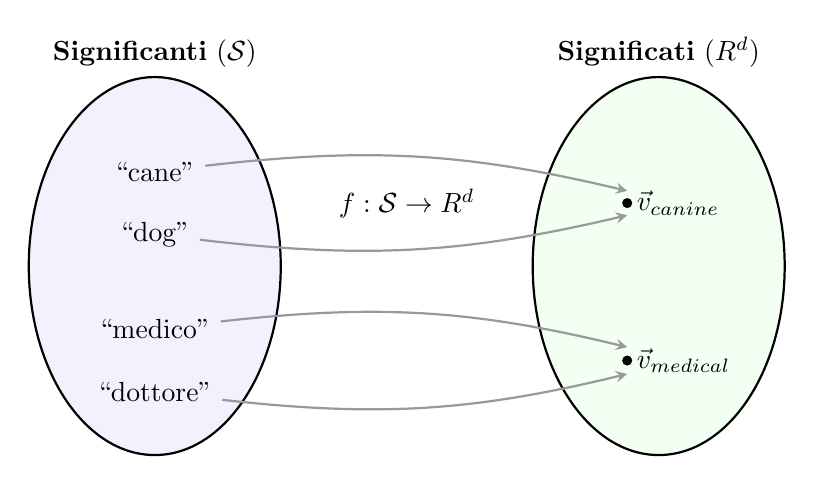
\begin{tikzpicture}[scale=0.8]
    % Insieme dei Significanti (Simboli)
    \draw[thick, fill=blue!5] (-4,0) ellipse (2cm and 3cm);
    \node[anchor=south] at (-4,3) {\textbf{Significanti} ($\mathcal{S}$)};
    \node (s1) at (-4,1.5) {``cane''};
    \node (s2) at (-4,0.5) {``dog''};
    \node (s3) at (-4,-1) {``medico''};
    \node (s4) at (-4,-2) {``dottore''};

    % Insieme dei Significati (Spazio Semantico)
    \draw[thick, fill=green!5] (4,0) ellipse (2cm and 3cm);
    \node[anchor=south] at (4,3) {\textbf{Significati} ($\mathbb{R}^d$)};
    
    % Punti nello spazio semantico
    \filldraw (3.5,1) circle (2pt) node[anchor=west] (v1) {$\vec{v}_{\text{canine}}$};
    \filldraw (3.5,-1.5) circle (2pt) node[anchor=west] (v2) {$\vec{v}_{\text{medical}}$};

    % Frecce di Mapping
    \draw[->, >=stealth, thick, gray!80] (s1) to [bend left=10] (v1);
    \draw[->, >=stealth, thick, gray!80] (s2) to [bend right=10] (v1);
    \draw[->, >=stealth, thick, gray!80] (s3) to [bend left=10] (v2);
    \draw[->, >=stealth, thick, gray!80] (s4) to [bend right=10] (v2);

    \node at (0,1) {$f: \mathcal{S} \to \mathbb{R}^d$};

\end{tikzpicture}
\caption{Rappresentazione del mapping tra lo spazio discreto dei simboli (Significanti) e lo spazio continuo dei vettori (Significati). L'obiettivo è apprendere una funzione $f$ tale che simboli diversi con significati simili vengano proiettati in vettori vicini nello spazio matematico.}
\label{fig:signifier_signified_mapping}
\end{figure}
Apprendere questa relazione è la \textit{conditio sine qua non} per permettere alle macchine di manipolare i simboli non solo come sequenze di bit, ma come entità portatrici di senso. Senza questo passaggio, il ragionamento logico e la coerenza semantica rimarrebbero preclusi.
\subsubsection{Gli assi del linguaggio}
\label{subsubsec:linguistic_axes}
\begin{figure}[h!]
    \centering
    \includegraphics[width=0.6\textwidth]{pictures/cap3/Ferdinand_de_Saussure_by_Jullien.png}
    \caption{Ferdinand de Saussure, fondatore della linguistica strutturale e teorico dei rapporti sintagmatici e associativi (paradigmatici) del linguaggio \cite{saussure_wikipedia_image}.}
    \label{fig:saussure}
\end{figure}
Per addestrare modelli capaci di catturare i significati dai significanti, li si pone nella condizione di analizzare enormi corpora di testo attraverso le due dimensioni fondamentali lungo le quali si articola ogni lingua: gli \textbf{assi saussuriani}.
\begin{figure}[htbp]
    \centering
    \tikzset{
        mainword/.style={font=\large\bfseries, text=black},
        altword/.style={font=\small\itshape, text=gray},
        axislabel/.style={font=\sffamily\bfseries\small},
        question/.style={font=\scriptsize\itshape, text=black!70, align=center}
    }
    \begin{tikzpicture}[>=LaTeX, node distance=1.5cm]
        % Assi
        \draw[->, thick, black!50] (-4, 0) -- (6, 0);
        \draw[->, thick, black!50] (0, -3.5) -- (0, 3.5);

        % Centro (Parola Target)
        \node[draw=black, thick, fill=white, inner sep=5pt] (target) at (0,0) {\textbf{mangia}};

        % Asse Sintagmatico (Orizzontale)
        \node[mainword] (w_prev2) at (-3, 0) {Il};
        \node[mainword] (w_prev1) at (-1.5, 0) {gatto};
        \node[mainword] (w_next1) at (1.5, 0) {la};
        \node[mainword] (w_next2) at (3, 0) {mela};

        % Asse Paradigmatico (Verticale)
        \node[altword] at (0, 1.2) {osserva};
        \node[altword] at (0, 2.0) {rincorre};
        \node[altword] at (0, 2.8) {annusa};
        \node[altword] at (0, -1.2) {divora};
        \node[altword] at (0, -2.0) {gusta};

        % Etichette
        \node[axislabel, anchor=north east] at (6, -0.2) {Asse Sintagmatico};
        \node[question, anchor=north east] at (6, -0.7) {«Quale parola segue?»\\(Combinazione)};
        \node[axislabel, anchor=south] at (0, 3.6) {Asse Paradigmatico};
        \node[question, anchor=south] at (0, 4.0) {«Cosa potrei mettere al posto di...?»\\(Selezione)};
    \end{tikzpicture}
    \caption{Rappresentazione degli assi del linguaggio. L'asse orizzontale mostra la sequenza lineare (sintagma), quello verticale le alternative possibili (paradigma).}
    \label{fig:linguistic_axes}
\end{figure}

L'\textbf{asse sintagmatico} riguarda la \textbf{combinazione}: risponde alla domanda \textit{«Quale parola segue?»} e governa la creazione di catene lineari (frasi). Al contrario, l'\textbf{asse paradigmatico} riguarda la \textbf{selezione}: risponde alla domanda \textit{«Cosa potrei mettere al posto di questa parola?»}. 
Gli algoritmi di embedding estraggono valore proprio all'intersezione di questi assi: analizzano le catene \textbf{sintagmatiche} osservabili nel testo per ricostruire lo spazio \textbf{paradigmatico} delle somiglianze. In fase di addestramento, il modello valuta quali termini siano intercambiabili in un dato contesto, mentre in fase di generazione opera sulla catena sintagmatica costruendo una sequenza coerente. È questa danza tra selezione e combinazione che permette l'emergere della coerenza semantica nei modelli moderni.

\subsubsection{L'ipotesi distribuzionale}
\label{subsubsec:distributional_hypothesis}

Per costruire queste relazioni di significato è necessario partire da un'ipotesi fondamentale. Supponiamo di non conoscere il significato della parola \textit{ongchoi}, ma di incontrarla nei seguenti contesti:

\begin{enumerate}
    \item \textit{L'ongchoi è deliziosa saltata con aglio.}
    \item \textit{L'ongchoi è ottima servita con riso.}
    \item \textit{...foglie di ongchoi con salse salate...}
\end{enumerate}

Ora immaginiamo di aver già visto molte di queste parole-contesto in altri esempi, come:

\begin{enumerate}
    \item \textit{...gli spinaci saltati con aglio serviti sul riso...}
    \item \textit{...le coste, con i loro gambi e foglie, sono molto gustose...}
    \item \textit{...il cavolo riccio e altre verdure a foglia dal sapore salato...}
\end{enumerate}

Il fatto che \textit{ongchoi} compaia insieme a parole come \textit{riso}, \textit{aglio}, \textit{deliziosa} e \textit{salata}, proprio come \textit{spinaci}, \textit{coste} o \textit{cavolo riccio}, suggerisce che l'ongchoi sia una verdura a foglia simile a queste altre verdure. Questo è il principio dell'ipotesi distribuzionale per il quale parole semanticamente simili tendono a comparire in contesti simili.

\begin{notebox}
\textbf{Ipotesi Distribuzionale}\\
Si definisce ipotesi distribuzionale quella ipotesi per la quale parole simili compaiono in contesti simili. 
\end{notebox}

Tale ipotesi suggerisce che il significato delle parole venga appreso sulla base del contesto in cui queste appaiono. Se questa intuizione viene seguita, allora diventa possibile assegnare rappresentazioni numeriche alle parole sulla base della loro occorrenza in contesti specifici. Prima di arrivare però a capire come costruire gli embeddings è necessario introdurre una ulteriore intuizione attribuita ad Osgood nel 1957.

\subsubsection{Ipotesi di Osgood: il significato come vettore}
\label{subsubsec:osgood_hypothesis}

Un contributo fondamentale alla rappresentazione del significato proviene dal lavoro di Osgood \parencite{Osgood1957Measurement}, che studiò la componente affettiva delle parole. Osgood mostrò che i giudizi emotivi associati a una parola possono essere descritti lungo tre dimensioni principali:

\begin{enumerate}
    \item \textbf{Valenza}: quanto la parola è percepita come positiva o negativa.
    \item \textbf{Arousal}: quanto la parola induce attivazione emotiva.
    \item \textbf{Dominanza}: quanto la parola implica controllo o sottomissione.
\end{enumerate}

Ogni parola può quindi essere rappresentata come una tripla di valori numerici che ne definiscono la posizione in questo spazio tridimensionale. Ad esempio:
\[
\textit{heartbreak} \rightarrow [2.5,\ 5.7,\ 3.6]
\]

L'intuizione rivoluzionaria di Osgood è la seguente:

\begin{notebox}
\textbf{Ipotesi di Osgood}\\
Il significato di una parola può essere rappresentato come un vettore in uno spazio semantico.
\end{notebox}

Questa idea è stata la prima ad anticipare direttamente i moderni modelli di \textit{word embeddings}, in cui ogni parola è descritta come un punto in uno spazio multidimensionale corrispondente a un significato. Mentre Osgood lavorava con tre dimensioni interpretabili psicologicamente, i modelli computazionali moderni utilizzano centinaia o migliaia di dimensioni apprese automaticamente dai dati, catturando relazioni semantiche complesse che vanno ben oltre la dimensione affettiva.

\subsubsection{Verso i word embeddings}
\label{subsubsec:towards_embeddings}
L'unione dell'ipotesi distribuzionale e dell'ipotesi di Osgood ha aperto la strada agli embeddings come modello fondamentale per la rappresentazione computazionale del significato. Da un lato, l'ipotesi distribuzionale fornisce il principio secondo cui il significato delle parole può essere inferito dai contesti in cui esse compaiono; dall'altro, l'ipotesi di Osgood suggerisce che tale significato possa essere rappresentato come un vettore numerico in uno spazio semantico.
Nelle sezioni successive introdurremo le principali famiglie di embeddings, partendo dai modelli basati su conteggi (count-based) fino ai moderni embeddings contestuali prodotti da architetture Transformer. Per orientare il lettore, è utile chiarire fin da subito le principali tipologie di embeddings che verranno introdotte nel seguito.
In base alla natura della rappresentazione prodotta, è possibile distinguere due grandi famiglie: embeddings \textbf{statici} ed embeddings \textbf{dinamici}.
\begin{figure}[htbp]
\centering
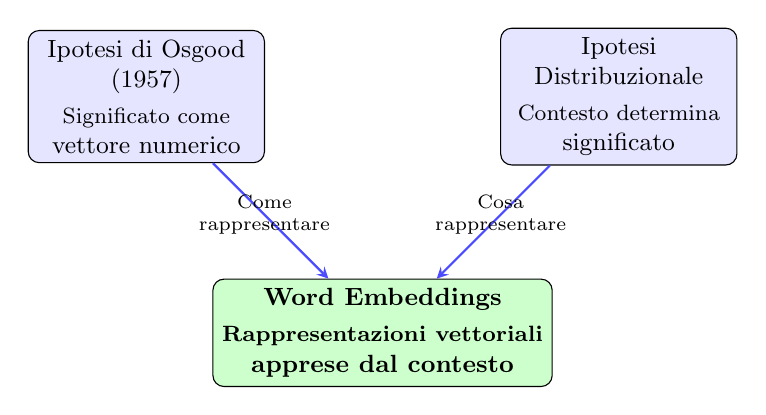
\begin{tikzpicture}[
    node distance=2cm,
    box/.style={draw, rectangle, rounded corners, minimum width=3cm, minimum height=1cm, align=center, font=\small, fill=blue!10},
    result/.style={draw, rectangle, rounded corners, minimum width=4cm, minimum height=1.2cm, align=center, font=\small\bfseries, fill=green!20},
    arrow/.style={->, >=stealth, thick}
]
    % Ipotesi di partenza
    \node[box] (osgood) at (-3, 2) {Ipotesi di Osgood\\(1957)\\[0.2em]\footnotesize Significato come\\vettore numerico};
    
    \node[box] (distributional) at (3, 2) {Ipotesi\\Distribuzionale\\[0.2em]\footnotesize Contesto determina\\significato};
    
    % Risultato
    \node[result] (embeddings) at (0, -1) {Word Embeddings\\[0.2em]\footnotesize Rappresentazioni vettoriali\\apprese dal contesto};
    
    % Frecce convergenti
    \draw[arrow, blue!70] (osgood) -- (embeddings);
    \draw[arrow, blue!70] (distributional) -- (embeddings);
    
    % Etichette sulle frecce
    \node[font=\scriptsize, text width=2cm, align=center] at (-1.5, 0.5) {Come\\rappresentare};
    \node[font=\scriptsize, text width=2cm, align=center] at (1.5, 0.5) {Cosa\\rappresentare};

\end{tikzpicture}
\caption{Convergenza delle due ipotesi fondamentali negli embeddings moderni. L'ipotesi di Osgood fornisce il \emph{formato} della rappresentazione (vettori numerici), mentre l'ipotesi distribuzionale indica \emph{cosa} deve essere catturato (relazioni contestuali tra parole).}
\label{fig:convergenza_ipotesi}
\end{figure}
\begin{notebox}
\textbf{Embeddings statici}\\
Si definisce statico un embedding in cui ogni parola del vocabolario è associata a un unico vettore pre-computato. Tale rappresentazione rimane invariata a prescindere dal contesto specifico in cui la parola appare.
\end{notebox}
Negli embeddings statici, a ciascun tipo di parola del vocabolario è associato un unico vettore, indipendente dal contesto in cui la parola appare. Questa categoria include sia gli embeddings distribuzionali basati su conteggi, come le matrici termine--documento e termine--termine eventualmente ridotte tramite SVD, sia gli embeddings predittivi appresi mediante modelli neurali, come Word2Vec.
\begin{notebox}
\textbf{Embeddings dinamici (Contestuali)}\\
Si definisce dinamico un embedding in cui la rappresentazione vettoriale di una parola viene computata in modo dipendente dal contesto, come funzione dell'intera sequenza di input. La stessa parola riceve quindi vettori diversi a seconda del contesto semantico e sintattico in cui compare.\end{notebox}
Gli embeddings dinamici, o contestuali, producono invece una rappresentazione dipendente dal contesto: la stessa parola può essere associata a vettori diversi a seconda della frase in cui compare. Tali rappresentazioni sono generate da modelli di linguaggio neurali profondi, a partire da architetture ricorrenti fino ai moderni modelli Transformer, come BERT.
\begin{figure}[htbp]
\centering
\begin{forest}
  for tree={
    draw,
    rounded corners,
    fill=blue!5,
    align=center,
    font=\small,
    edge={->, thick},
    l sep=1.2cm,    
    s sep=0.5cm,
    inner sep=6pt
  }
  [\textbf{Embeddings}
    [\textbf{Statici}
      [{\textbf{Count-based}\\(Term-Doc, Term-Term)}]
      [{\textbf{Predittivi neurali}\\(Word2Vec, GloVe)}]
    ]
    [\textbf{Dinamici}
      [{\textbf{Modelli neurali profondi}\\(ELMo, BERT, GPT)}]
    ]
  ]
\end{forest}
\caption{Classificazione delle principali tipologie di embeddings trattate nel capitolo.}
\label{fig:classificazione_embeddings}
\end{figure}
La Figura~\ref{fig:classificazione_embeddings} riassume questa tassonomia. Nelle sezioni successive analizzeremo in dettaglio ciascuna di queste famiglie, comprendendo come si costruiscono, quali proprietà possiedono e quali limiti presentano. Questo percorso ci condurrà fino agli embeddings densi prodotti da modelli come BERT, che costituiscono l'input degli Sparse Autoencoders discussi nel Capitolo~\ref{sec:04_disentangling_dense_embeddings_with_sparse_autoencoders}.
\subsection{Embeddings statici}
\label{sec:static_embeddings}
In questa sezione introduciamo gli embeddings statici, rappresentazioni in cui ogni parola del vocabolario è associata a un unico vettore fisso, indipendente dal contesto in cui compare. Distingueremo tra due approcci fondamentali: i metodi \textbf{count-based}, che costruiscono rappresentazioni a partire da statistiche di co-occorrenza, e i metodi \textbf{predittivi}, che apprendono embeddings tramite reti neurali addestrate a predire parole in contesto.
\subsubsection{Embeddings count-based}
\label{subsubsec:count_based}
Il modo più semplice per costruire embeddings vettoriali delle parole è basato sulla \textbf{matrice di co-occorrenza}, una struttura che codifica quante volte determinati elementi linguistici compaiono insieme all'interno di un corpus. Esistono diverse varianti di matrici di co-occorrenza; in questa sezione ne introduciamo due fondamentali: la \emph{term-document matrix} e la \emph{term-term matrix}.
\paragraph{Matrice termine-documento.}
In una matrice termine-documento ogni riga rappresenta una parola del vocabolario e ogni colonna rappresenta un documento appartenente a una collezione di testi. Ogni cella della matrice contiene il numero di volte in cui la parola associata alla riga compare nel documento associato alla colonna. Un esempio di term-document matrix è riportato nella Tabella~\ref{tab:term_document_shakespeare}, che mostra le occorrenze di quattro parole in quattro opere di Shakespeare.

\begin{table}[h!]
\centering
\begin{tabular}{lcccc}
\hline
 & \textbf{As You Like It} & \textbf{Twelfth Night} & \textbf{Julius Caesar} & \textbf{Henry V} \\
\hline
battle & 1   & 0  & 7  & 13 \\
good   & 114 & 80 & 62 & 89 \\
fool   & 36  & 58 & 1  & 4  \\
wit    & 20  & 15 & 2  & 3  \\
\hline
\end{tabular}
\caption{Term-document matrix per quattro parole in quattro opere di Shakespeare. Ogni cella contiene il numero di occorrenze della parola (riga) nel documento (colonna).}
\label{tab:term_document_shakespeare}
\end{table}
Questa matrice può essere interpretata in due modi distinti ma complementari. Se si considerano le \textbf{colonne} della matrice, ciascun documento è rappresentato come un vettore in uno spazio di dimensione $|V|$, dove $|V|$ è la dimensione del vocabolario. Tale rappresentazione costituisce il fondamento del \emph{vector space model} per il recupero dell'informazione. 
Alternativamente, se si considerano le \textbf{righe} della matrice, ogni parola può essere interpretata come un vettore in uno spazio di dimensione pari al numero di documenti.
\begin{notebox}
\textbf{Interpretazione delle righe della matrice termine-documento}\\
Due parole risultano simili se presentano distribuzioni simili sui documenti, ovvero se tendono a comparire negli stessi testi con frequenze comparabili.
\end{notebox}
La term-document matrix fornisce quindi una prima, semplice forma di \emph{embedding distribuzionale} delle parole, in cui il significato emerge dalla loro distribuzione nei documenti del corpus.
\paragraph{Matrice termine-termine.}
Un'alternativa alla matrice termine--documento per la rappresentazione distribuzionale delle parole è la matrice termine-termine, detta anche \emph{word--word matrix} o \emph{term--context matrix}. In questo caso, le colonne della matrice non sono più etichettate da documenti, bensì da parole del vocabolario. La matrice ha quindi dimensionalità $|V| \times |V|$, dove $|V|$ indica la dimensione del vocabolario.
In una matrice termine-termine, ogni riga rappresenta una \textbf{parola target} e ogni colonna rappresenta una \textbf{parola di contesto}. Ciascuna cella contiene il numero di volte in cui la parola di contesto compare nel contesto della parola target all'interno di un corpus di addestramento. Il concetto di \emph{contesto} viene tipicamente definito tramite una \textbf{finestra scorrevole} attorno alla parola target. Ad esempio, fissata una finestra di ampiezza $\pm k$, una parola è considerata di contesto se compare entro $k$ posizioni a sinistra o a destra della parola target nel testo.
La Tabella~\ref{tab:term_term_wikipedia} riporta un estratto reale di una matrice termine--termine calcolata sul corpus Wikipedia.
\begin{table}[h!]
\centering
\begin{tabular}{lcccccc}
\hline
\textbf{Parola} & \textbf{aardvark} & \textbf{computer} & \textbf{data} & \textbf{result} & \textbf{pie} & \textbf{sugar} \\
\hline
cherry       & 0 & 2    & 8    & 9    & 442 & 25 \\
strawberry   & 0 & 0    & 0    & 1    & 60  & 19 \\
digital      & 0 & 1670 & 1683 & 85   & 5   & 4  \\
information  & 0 & 3325 & 3982 & 378  & 5   & 13 \\
\hline
\end{tabular}
\caption{Estratto di una matrice termine--termine calcolata sul corpus Wikipedia. Ogni cella contiene il numero di co-occorrenze tra la parola target (riga) e la parola di contesto (colonna) all'interno di una finestra di contesto locale.}
\label{tab:term_term_wikipedia}
\end{table}
In questa rappresentazione, ogni parola è associata a un vettore in uno spazio di dimensione $|V|$, in cui ciascuna dimensione corrisponde a una parola di contesto. Parole semanticamente simili tendono ad avere vettori simili, poiché compaiono in contesti linguistici analoghi.
\begin{notebox}
\textbf{Interpretazione della matrice termine--termine}\\
Due parole risultano semanticamente simili se presentano vettori di co-occorrenza simili, ovvero se tendono a comparire negli stessi contesti linguistici, anche nel caso in cui non compaiano mai direttamente insieme.
\end{notebox}
Data $|V|$ la dimensione del vocabolario, tale matrice ha una dimensionalità $|V| \times |V|$. Si hanno tuttavia due problemi:
\begin{enumerate}
    \item Dal momento che ogni parola co-occorrerà solo con pochissime altre, \textit{la dimensionalità della matrice è enorme}.
    \item La maggior parte delle celle è nulla, e quindi \textit{i vettori sono estremamente sparsi}.
\end{enumerate}
Per affrontare questi problemi esistono diverse strategie, tra cui la riduzione dimensionale tramite SVD e il passaggio a paradigmi predittivi come Word2Vec.
\paragraph{Riduzione dimensionale tramite SVD.}
Un metodo per la riduzione della dimensionalità è la Singular Value Decomposition applicata alla word--context matrix. Sia $M \in \mathbb{R}^{|V| \times |V|}$ la word--context matrix, eventualmente pesata tramite tf-idf. La decomposizione ai valori singolari consente di fattorizzare $M$ come prodotto di tre matrici:
\[
M = U \Sigma V^\top
\]
dove $U$ e $V$ sono matrici ortogonali e $\Sigma$ è una matrice diagonale contenente i valori singolari ordinati in modo decrescente. Per ottenere una rappresentazione a dimensionalità ridotta, si considera una versione troncata della decomposizione, mantenendo solo i primi $k$ valori singolari:
\[
M \approx U_k \Sigma_k V_k^\top
\]
con $k \ll |V|$. Le righe della matrice $U_k \Sigma_k$ costituiscono una rappresentazione densa delle parole target in uno spazio latente di dimensione $k$. In questo nuovo spazio, ogni parola è descritta da un vettore a dimensionalità ridotta, in cui le correlazioni semantiche risultano più evidenti rispetto alla rappresentazione originale sparsa.
\paragraph{Cosine similarity.}
Una volta ottenuti vettori di embedding (sia da matrici di co-occorrenza sia da riduzione dimensionale), serve una metrica per quantificare la similarità semantica tra parole. La \textbf{cosine similarity} è una misura di similarità tra vettori che valuta il coseno dell'angolo compreso tra essi nello spazio vettoriale. Data la sua indipendenza dalla lunghezza dei vettori, risulta particolarmente adatta a confrontare vettori di frequenze o di pesi.
Dati due vettori $u$ e $v$, la similarità coseno è definita come:
\begin{equation}
\text{cosine\_sim}(u, v) = 
\frac{u \cdot v}{\|u\| \, \|v\|}
= \frac{\sum_i u_i v_i}{\sqrt{\sum_i u_i^2} \, \sqrt{\sum_i v_i^2}}.
\end{equation}
Il valore risultante è compreso tra $-1$ e $1$: $1$ indica massima similarità (stessa direzione), $0$ indica ortogonalità (nessuna similarità), e valori negativi indicano direzioni opposte. Nelle applicazioni di NLP la cosine similarity è spesso preferita alla distanza Euclidea, perché ci interessa confrontare il \textit{pattern} delle co-occorrenze piuttosto che le loro magnitudini assolute.
\subsubsection{Word2Vec: un approccio predittivo}
\label{subsubsec:word2vec}
\begin{figure}[htbp]
\centering
\begin{tikzpicture}[
    node distance=0.8cm,
    theory/.style={draw, ellipse, minimum width=2.5cm, minimum height=1cm, align=center, font=\footnotesize, fill=blue!10},
    impl/.style={draw, rectangle, rounded corners, minimum width=2.5cm, minimum height=0.8cm, align=center, font=\footnotesize, fill=green!15}
]
    % Colonna sinistra: Osgood
    \node[theory] (osg_theory) at (-3, 3.5) {
        \textbf{Osgood}\\
        {\scriptsize Significato $\to$ vettore}
    };
    
    \node[impl] (osg_vectors) at (-3, 2) {
        Matrici $W$, $C$\\
        $\mathbf{w}, \mathbf{c} \in \mathbb{R}^d$
    };
    
    \node[impl] (osg_sim) at (-3, 0.8) {
        Similarità:\\
        $\mathbf{w} \cdot \mathbf{c}$
    };
    
    % Colonna destra: Distribuzionale
    \node[theory] (dist_theory) at (3, 3.5) {
        \textbf{Distribuzionale}\\
        {\scriptsize Contesto $\to$ significato}
    };
    
    \node[impl] (dist_window) at (3, 2) {
        Finestra $\pm k$\\
        Contesto locale
    };
    
    \node[impl] (dist_cooc) at (3, 0.8) {
        Co-occorrenze\\
        $P(c \mid w)$
    };
    
    % Frecce
    \draw[->, thick, blue!60] (osg_theory) -- (osg_vectors);
    \draw[->, thick, blue!60] (osg_vectors) -- (osg_sim);
    \draw[->, thick, blue!60] (dist_theory) -- (dist_window);
    \draw[->, thick, blue!60] (dist_window) -- (dist_cooc);
    
    % Word2Vec al centro in basso
    \node[draw, rectangle, rounded corners, fill=orange!20, minimum width=7cm, minimum height=1cm, align=center, font=\small\bfseries] (w2v) at (0, -0.8) {
        Word2Vec\\
        {\footnotesize $\max \sum \log \sigma(\mathbf{w} \cdot \mathbf{c})$ per $(w,c)$ in finestra $k$}
    };
    
    \draw[->, thick, gray] (osg_sim) -- (w2v);
    \draw[->, thick, gray] (dist_cooc) -- (w2v);

\end{tikzpicture}
\caption{Word2Vec come fusione tra teoria e implementazione. A sinistra, l'ipotesi di Osgood si traduce nella scelta di vettori continui e nel prodotto scalare come misura di similarità. A destra, l'ipotesi distribuzionale si concretizza nella finestra di contesto e nella modellazione di co-occorrenze. Word2Vec unifica elegantemente queste due linee, apprendendo vettori che massimizzano la predizione di co-occorrenze locali.}
\label{fig:word2vec_teoria_implementazione}
\end{figure}
Sebbene i metodi basati su conteggi e la riduzione dimensionale tramite SVD permettano di ottenere rappresentazioni semanticamente dense, essi presentano limiti strutturali non trascurabili. Il calcolo della decomposizione ai valori singolari su matrici di co-occorrenza è computazionalmente oneroso, con una complessità che cresce sensibilmente rispetto alla dimensione del vocabolario, rendendo difficile la scalabilità su corpora massicci.
Per superare queste criticità, Mikolov et al. hanno introdotto \textit{Word2Vec} \parencite{mikolov2013efficientestimationwordrepresentations}, un framework basato su un paradigma radicalmente diverso: la \textbf{predizione}. Invece di riassumere statistiche globali, Word2Vec apprende gli embeddings processando il testo localmente. Lo spostamento di paradigma risiede nel fatto che, anziché contare le occorrenze totali, addestriamo un classificatore su un compito di \textbf{classificazione binaria}. Il modello deve rispondere alla domanda:
\begin{center}
\textit{``Data la parola target $w$ (es. \textit{albicocca}), qual è la probabilità che la parola candidata $c$ (es. \textit{marmellata}) compaia nel suo contesto?''}
\end{center}
In questo approccio, noto come \textbf{self-supervision}, il testo stesso fornisce le etichette: ogni parola $c$ che appare effettivamente vicino a $w$ nel corpus fornisce un esempio positivo (etichetta $1$), dovo per ``vicino" si intende dentor una finstra di contesto di $k$ parole. Al contrario, per addestrare il classificatore, il modello genera artificialmente degli esempi negativi campionando parole casuali dal vocabolario che non compaiono nel contesto di $w$ (etichetta $1$).
\paragraph{Il classificatore e la funzione sigmoide.}
L'intuizione alla base del classificatore è che due parole siano semanticamente vicine se i loro vettori di embedding sono simili. Per misurare questa affinità, utilizziamo il \textbf{prodotto scalare} tra il vettore della parola target $\mathbf{w}$ e il vettore della parola di contesto $\mathbf{c}$:
\[
\text{Similarity}(w,c) \approx \mathbf{w} \cdot \mathbf{c}
\]

Poiché il prodotto scalare può assumere qualsiasi valore reale, utilizziamo la funzione \textbf{sigmoide} $\sigma(x)$ per mappare il risultato in una probabilità compresa tra $0$ e $1$:
\begin{equation}
\sigma(x) = \frac{1}{1 + e^{-x}}
\end{equation}

Il modello stima quindi la probabilità che la coppia $(w, c)$ sia un esempio positivo ($+$) come:
\begin{equation}
P(+ \mid w, c) = \sigma(\mathbf{w} \cdot \mathbf{c}) = \frac{1}{1 + e^{-\mathbf{w} \cdot \mathbf{c}}}
\end{equation}

Nel caso generale, data una parola target $w$ e un'intera finestra di $L$ parole di contesto $c_{1:L}$, il modello assume che le parole nel contesto siano indipendenti tra loro. La probabilità complessiva è dunque data dal prodotto delle probabilità individuali:
\begin{equation}
\log P(+ \mid w, c_{1:L}) = \sum_{i=1}^L \log \sigma(\mathbf{w} \cdot \mathbf{c}_i)
\end{equation}

\paragraph{Perché due matrici? Il ruolo di $W$ e $C$.}
Una caratteristica distintiva di Word2Vec è il mantenimento di \textit{due rappresentazioni distinte} per ogni parola, organizzate in due matrici di pesi separate (Figura~\ref{fig:skipgram_structure}). Una matrice $W$ relativa alle parole target che contiene i vettori utilizzati quando la parola è il centro della finestra, e una matrice $C$ che contiene i vettori utilizzati quando la parola appare nel contesto di un'altra o viene estratta come esempio negativo.

\begin{figure}[h!]
    \centering
    \includegraphics[width=0.7\textwidth]{pictures/embeddings_w2vec.png}
    \caption{Lo skip-gram apprende in totale due insiemi di embedding, uno per i target ($W$) e uno per i contesti ($C$), per un totale di $2|V|$ vettori. L'addestramento mira a massimizzare la probabilità che parole vicine nel testo abbiano vettori simili.}
    \label{fig:skipgram_structure}
\end{figure}

Sdoppiando le matrici, il modello garantisce la \textit{stabilità dell'ottimizzazione}. Se usassimo un unico vettore $\mathbf{v}$, il modello cercherebbe di massimizzare il prodotto scalare $\mathbf{v} \cdot \mathbf{v}$ (auto-similarità), portando i valori a crescere all'infinito. Con due matrici, il modello apprende relazioni distribuzionali senza questo vincolo. Al termine, si utilizzano solitamente i vettori di $W$ o la media $W+C$.
\paragraph{Finestra di contesto e precisione semantica.}
L'ampiezza della finestra di contesto $k$ controlla quanta informazione sintagmatica il modello può sfruttare per inferire il paradigma semantico. All'aumentare di $k$, il modello osserva un contesto più ampio e cattura relazioni semantiche progressivamente più ricche.
\begin{itemize}
    \item \textit{Finestra stretta} ($k$ piccolo): il contesto è locale e cattura principalmente regolarità \textit{funzionali e sintattiche}. Gli embeddings risultanti tendono a raggruppare parole che svolgono ruoli grammaticali simili.
    \item \textit{Finestra ampia} ($k$ grande): il contesto include indizi più distanti, catturando affinità \textit{semantiche e tematiche}. Ad esempio, parole come \textit{ospedale} e \textit{medico} non sono intercambiabili sintatticamente, ma co-occorrono in ambienti discorsivi simili e risultano quindi vicine nello spazio vettoriale.
\end{itemize}
Questa relazione tra ampiezza della finestra e tipo di similarità catturata riflette direttamente il principio degli assi saussuriani: osservando porzioni più ampie della catena sintagmatica, il modello ricostruisce con maggiore precisione lo spazio paradigmatico delle sostituzioni semanticamente plausibili.
\paragraph{Geometria dell'analogia: il modello del parallelogramma.}
Quando lo spazio latente è coerente, non si limita a raggruppare parole simili: tende anche a codificare \textit{relazioni} come direzioni stabili. Questo si manifesta nel ragionamento analogico, spesso descritto tramite il cosiddetto modello del parallelogramma. 

\begin{notebox}
\textbf{Modello del parallelogramma}\\
Le relazioni semantiche possono essere codificate come differenze vettoriali approssimativamente costanti. Data l'analogia «$a$ sta ad $a^*$ come $b$ sta ad $b^*$» (es.\ \textit{uomo}:\textit{donna} = \textit{re}:\textit{regina}), il termine incognito $b^*$ è approssimabile come:
\[ b^* \approx b - a + a^* \]
\end{notebox}

\begin{figure}[htbp]
\centering
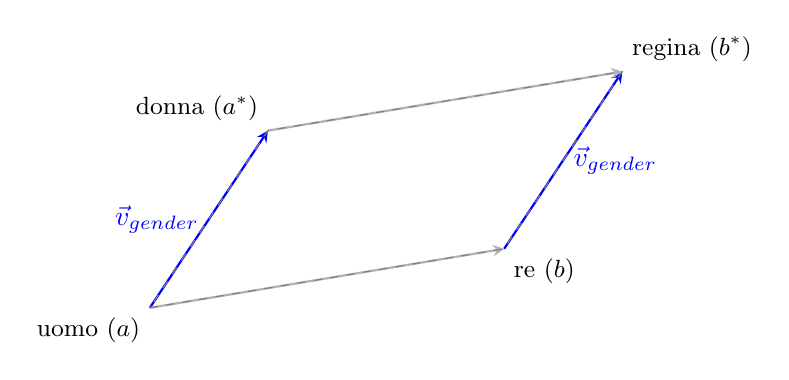
\begin{tikzpicture}[scale=1.5, >=stealth]
    \coordinate (man) at (0,0);
    \coordinate (woman) at (1,1.5);
    \coordinate (king) at (3,0.5);
    \coordinate (queen) at (4,2);

    \draw[->, thick, blue] (man) -- (woman) node[midway, left] {$\vec{v}_{gender}$};
    \draw[->, thick, blue] (king) -- (queen) node[midway, right] {$\vec{v}_{gender}$};
    \draw[->, thick, gray!60] (man) -- (king);
    \draw[->, thick, gray!60] (woman) -- (queen);

    \node[below left] at (man) {\small uomo ($a$)};
    \node[above left] at (woman) {\small donna ($a^*$)};
    \node[below right] at (king) {\small re ($b$)};
    \node[above right] at (queen) {\small regina ($b^*$)};

    \draw[dashed, gray] (man) -- (king) -- (queen) -- (woman) -- cycle;
\end{tikzpicture}
\caption{Rappresentazione geometrica del modello del parallelogramma nello spazio latente.}
\label{fig:parallelogramma}
\end{figure}

\subsubsection{Limiti degli embeddings statici}
\label{subsubsec:static_limits}
La logica ``più sintagma $\Rightarrow$ paradigma più preciso'' evidenzia però un limite intrinseco di Word2Vec: anche se durante l'addestramento sfrutta il contesto, il risultato finale è un \textbf{embedding statico}. Una volta appresi i vettori, ogni parola è associata a un'unica rappresentazione, indipendente dall'uso concreto in frase. Questo comporta almeno due criticità fondamentali:
\begin{enumerate}
    \item \textit{Polisemia:} una parola con più sensi (es.\ \textit{banco} come mobile o come istituzione finanziaria) viene compressa in un unico vettore che media usi diversi, riducendo la precisione semantica proprio dove il contesto dovrebbe aiutare.
    \item \textit{Contesto ``dimenticato'' in inferenza:} Word2Vec usa la finestra sintagmatica per \emph{apprendere} i vettori, ma in \textit{inferenza} l'embedding di una parola è recuperato come valore fisso dal dizionario del modello e non viene ricalcolato in funzione della frase specifica. Di conseguenza, la stessa parola mantiene lo stesso vettore anche in contesti diversi, e il contesto non può più agire da meccanismo di disambiguazione.
\end{enumerate}
\begin{notebox}
\textbf{Training vs inferenza}\\
Per \textbf{inferenza} si intende l'uso del modello \emph{dopo} l'addestramento: dati nuovi input, i parametri appresi $\theta$ restano fissi e il modello calcola solo le sue uscite. In Word2Vec, durante l'addestramento il contesto influenza l'apprendimento dei vettori; in inferenza, però, ogni parola ha un embedding fisso indipendente dal contesto in cui compare.
\end{notebox}

Se il significato di una parola dipende sistematicamente dalla ricchezza del sintagma che la circonda, allora la rappresentazione dovrebbe essere una \textbf{funzione del contesto}, non una costante. Questa osservazione motiva il passaggio agli \textbf{embeddings dinamici (contestuali)}: invece di limitarsi a una finestra fissa e a un vettore unico per parola, essi mirano a incorporare informazione proveniente dall'intera sequenza, generando un vettore diverso per ogni occorrenza. 
Per ottenere questo comportamento servono architetture in grado di modellare il linguaggio come flusso e memoria. Nella prossima sezione introdurremo brevemente le architetture ricorrenti e il meccanismo di attenzione, che preparano il terreno per i moderni Transformer e, in particolare, per BERT—il modello che produce gli embeddings densi su cui applicheremo gli Sparse Autoencoders nei capitoli successivi.




%%%%%%%%%%%%%%%%%%%%%%%%%%%%%%%%%%%%%%%%%%


\subsection{Embeddings dinamici (contestuali)}
\label{sec:dynamic_embeddings}
La sezione precedente ha chiarito un punto chiave: se un sintagma più ricco rende più preciso il paradigma, allora una rappresentazione che \emph{non} può sfruttare il contesto quando viene applicata a una frase concreta è inevitabilmente limitata. Gli embeddings statici (come quelli appresi da Word2Vec) usano il contesto in addestramento per stimare i vettori, ma poi restituiscono un dizionario di rappresentazioni fisse: in inferenza, l'embedding di una parola è sempre lo stesso, indipendentemente dalle parole che la circondano.
Questo limite diventa evidente nei casi di \textit{polisemia} e \textit{omonimia}. Parole come \textit{banco} (mobile vs istituzione finanziaria) o \textit{pesca} (frutto vs attività) vengono collassate in un unico punto dello spazio vettoriale, che finisce per rappresentare una ``media'' tra sensi diversi. Ma la tesi sintagma--paradigma suggerisce l'opposto: il senso corretto non è una proprietà isolata del token, bensì emerge dall'interazione con la catena sintagmatica in cui quel token è inserito.
Gli embeddings dinamici (o contestuali) rispondono esattamente a questa esigenza: invece di associare un vettore a un \emph{tipo} di parola (\textit{word type}), associano un vettore a una sua \emph{occorrenza} concreta (\textit{word instance}), calcolandolo come funzione del contesto in cui appare. In questo approccio, la rappresentazione non è più un parametro statico recuperato da una tabella di lookup, ma un risultato computazionale prodotto dal modello mentre elabora l'intera sequenza.
\begin{notebox}
\textbf{Embeddings contestuali}\\
Data una sequenza di token $x_1,\dots,x_n$, un embedding contestuale è una rappresentazione vettoriale $h_i$ per il token $x_i$ tale che
\[
h_i = f(x_i, x_{1:n}),
\]
dove $x_{1:n}$ rappresenta l'intera sequenza (contesto). A differenza degli embeddings statici, $h_i$ descrive un'istanza specifica della parola nel suo uso concreto (\textit{word instance}) e non la sua categoria astratta nel vocabolario (\textit{word type}).
\end{notebox}
In pratica, queste rappresentazioni emergono dagli \textbf{stati interni} di modelli neurali che processano sequenze. Un embedding statico è un parametro appreso e poi fissato; un embedding dinamico, invece, è l'\textbf{attivazione} della rete in \textbf{inferenza}: cambia se cambia il contesto. Per questo motivo, la stessa parola può corrispondere a vettori diversi in frasi diverse, perché il modello integra informazione sintattica e semantica dalle parole circostanti e disambigua il senso in modo implicito.
A questo punto la domanda diventa: \textit{come si cattura contesto su larga scala senza perdere informazione lungo la sequenza?} La storia recente delle architetture neurali per il linguaggio può essere letta come una sequenza di risposte progressive a questo vincolo. Nelle prossime sottosezioni introdurremo brevemente le principali tatappe di questa evoluzione: dalle reti ricorrenti al meccanismo di attenzione, fino ai Transformer che costituiscono la base dei moderni modelli linguistici.
\subsubsection{RNN e LSTM: memoria sequenziale}
\label{subsubsec:rnn_lstm_compendium}
Per produrre embeddings contestuali serve un'architettura che processi sequenze mantenendo ``memoria'' del passato. Le \textit{Reti Neurali Ricorrenti} (RNN) introducono connessioni cicliche che permettono di aggiornare uno stato nascosto $h_t$ incorporando informazione sia dal token corrente $x_t$ sia dallo stato precedente $h_{t-1}$:
\begin{equation}
h_t = g(Uh_{t-1} + Wx_t + b)
\end{equation}
dove $U$ e $W$ sono matrici di pesi, $b$ è un bias, e $g$ è una funzione di attivazione non lineare (tipicamente $\tanh$ o ReLU). In questo modo, lo stato $h_t$ accumula progressivamente informazione da tutti i token precedenti nella sequenza.
\begin{figure}[htbp]
\centering
\includegraphics[width=\textwidth]{pictures/rnn.png}
\caption{Illustrazione del funzionamento di una RNN. Ad ogni passo l'informazione contestuale viene passata a quello successivo attraverso lo stato nascosto $h_t$.}
\label{fig:rnn_flow}
\end{figure}
Tuttavia, le RNN classiche soffrono del problema del \textbf{vanishing gradient}: durante l'addestramento tramite \textit{backpropagation through time}, i gradienti vengono propagati all'indietro attraverso ogni passo temporale. Poiché il calcolo coinvolge moltiplicazioni ripetute della stessa matrice di pesi $U$, se i valori di questa matrice sono piccoli, il segnale del gradiente tende a ridursi esponenzialmente man mano che ci si allontana nel passato. Questo rende difficile apprendere dipendenze a lungo raggio: se una parola all'inizio della frase è cruciale per predire una parola alla fine, la RNN ``dimentica'' l'informazione iniziale perché il gradiente non riesce a trasportare l'errore così indietro nel tempo.
Le \textbf{LSTM} (Long Short-Term Memory) risolvono parzialmente questo problema tramite una struttura più complessa basata su \textbf{gate} (porte) che controllano esplicitamente quali informazioni mantenere, aggiornare o dimenticare. Senza entrare nei dettagli architetturali (disponibili in Appendice~\ref{app:lstm_details}), l'idea chiave è introdurre:
\begin{itemize}
    \item Un \textbf{forget gate} $f_t$ che decide quali informazioni dello stato precedente $c_{t-1}$ eliminare;
    \item Un \textbf{input gate} $i_t$ che decide quali nuove informazioni aggiungere;
    \item Un \textbf{output gate} $o_t$ che decide quali informazioni dello stato interno esporre come output $h_t$.
\end{itemize}
Questi meccanismi permettono alle LSTM di preservare meglio informazioni cruciali su sequenze lunghe, riducendo la degradazione del segnale. Lo stato nascosto $h_t$ di una LSTM può essere estratto come embedding contestuale: a differenza dell'embedding statico $e_t$ (che è una riga fissa di una matrice), il vettore $h_t$ integra informazione dall'intera storia fino a quel punto.
\begin{notebox}
\textbf{Embedding contestuale nelle RNN/LSTM}\\
In una RNN o LSTM, il vettore $h_t$ costituisce l'embedding contestuale della parola $w_t$. A differenza dell'embedding statico $e_t$ (che è una semplice riga della matrice di embedding), il vettore $h_t$ è dinamico: esso integra informazioni riguardanti l'intera storia della frase fino a quel momento.
\end{notebox}
Per catturare contesto sia da sinistra sia da destra, si utilizzano \textbf{RNN bidirezionali} (Bi-RNN): si addestrano due reti distinte, una che processa la sequenza da sinistra a destra ($\overrightarrow{h}_t$) e una da destra a sinistra ($\overleftarrow{h}_t$). L'embedding contestuale finale si ottiene concatenando i due stati:
\begin{equation}
h_t^{bi} = [\overrightarrow{h}_t \oplus \overleftarrow{h}_t]
\end{equation}
Nonostante i miglioramenti introdotti dalle LSTM e dalle architetture bidirezionali, questi modelli rimangono \textbf{limitati dalla natura sequenziale del calcolo}: ogni stato dipende dal precedente, rendendo impossibile la parallelizzazione e limitando comunque la capacità di catturare dipendenze molto lunghe. Questo motiva l'introduzione di meccanismi più potenti: l'\textbf{attenzione} e, successivamente, i \textbf{Transformer}.
% Per dettagli architetturali completi su RNN e LSTM, si veda l'Appendice~\ref{app:lstm_details}.
\subsubsection{Encoder-Decoder e il problema del bottleneck}
\label{subsubsec:encoder_decoder_bottleneck}
Quando il compito richiede di trasformare un'intera sequenza in un'altra sequenza (traduzione automatica, riassunto, question answering), emerge un ulteriore vincolo strutturale. L'architettura \textbf{Encoder-Decoder} affronta questo problema separando comprensione e generazione in due moduli distinti:
\begin{enumerate}
    \item \textbf{Encoder}: una RNN/LSTM che processa l'input $X = (x_1,\dots,x_n)$ e produce una sequenza di stati nascosti $h_1^{(e)},\dots,h_n^{(e)}$. Nel modello classico, l'intera sequenza viene riassunta in un singolo vettore a dimensione fissa, spesso identificato con l'ultimo stato dell'encoder:
    \begin{equation}
    c = h_n^{(e)}
    \end{equation}
    Questo vettore $c$ è chiamato \textit{context vector}: dovrebbe contenere le informazioni necessarie per ricostruire, tradurre o generare coerentemente l'output.    
    \item \textbf{Decoder}: una seconda RNN/LSTM che, condizionata sul vettore di contesto $c$, genera l'output $Y = (y_1,\dots,y_m)$ un token alla volta in modo autoregressivo:
    \begin{equation}
    P(Y\mid X) = \prod_{t=1}^{m} P(y_t \mid y_{<t}, c)
    \end{equation}
\end{enumerate}
\begin{figure}[htbp]
    \centering
    \includegraphics[width=\textwidth]{pictures/bottleneck.png}
    \caption{Schema Encoder--Decoder: quando il contesto $c$ coincide con il solo stato nascosto finale dell'encoder, tutta l'informazione della sequenza sorgente deve attraversare un \emph{collo di bottiglia} rappresentazionale prima di essere utilizzata dal decoder.}
    \label{fig:encoder_decoder_bottleneck}
\end{figure}
Il punto critico dell'architettura è evidente: l'intera frase (potenzialmente lunga e ricca di dipendenze) viene compressa in un unico vettore $c \in \mathbb{R}^d$. Questa scelta introduce un vero e proprio \textbf{collo di bottiglia informativo}:
\begin{itemize}
    \item \textit{Compressione forzata}: All'aumentare della lunghezza e complessità dell'input, cresce la quantità di informazione che deve essere ``stipata'' in una dimensione fissa $d$.
    \item \textit{Sensibilità alla distanza}: Anche con LSTM, la rappresentazione finale tende a privilegiare informazione recente nella sequenza; dettagli importanti all'inizio possono attenuarsi o venire sovrascritti durante la ricorrenza.
    \item \textit{Difficoltà di allineamento}: In traduzione serve sapere \emph{quale parte} dell'input è rilevante per generare \emph{quel particolare} token di output. Un vettore unico $c$ non esplicita alcun allineamento fine-grained tra posizioni.
\end{itemize}
Questo limite è concettualmente analogo a quello discusso nel Capitolo~\ref{sec:autoencoders} sugli autoencoders: anche lì un input complesso viene proiettato in uno spazio latente di dimensione fissa, e il decoder tenta una ricostruzione a partire da tale compressione. Nel caso seq2seq, però, la pressione sullo spazio latente è ancora più marcata, perché la ricostruzione non riguarda ``lo stesso oggetto'' ma una sequenza diversa (es.\ tradotta), che richiede sia contenuto semantico sia informazione strutturale.
\subsubsection{Meccanismo di attenzione: superare il bottleneck}
\label{subsubsec:attention_mechanism}
Il bottleneck dell'encoder--decoder ricorrente deriva dal vincolo che l'unica informazione sull'input $X$ disponibile al decoder sia un singolo vettore $c$. Il \textbf{meccanismo di attenzione} risolve questo problema permettendo al decoder di accedere direttamente a \emph{tutti} gli stati nascosti dell'encoder, selezionando dinamicamente la parte più rilevante dell'input a ogni passo di generazione.
\begin{figure}[htbp]
\centering
\includegraphics[width=\textwidth]{pictures/attention_dynamic_context.png}
\caption{Nel meccanismo di attenzione, a ciascun passo di decodifica $i$ il decoder utilizza un contesto \emph{dinamico} $c_i$ (diverso per ogni token generato), calcolato come funzione di tutti gli stati nascosti dell'encoder.}
\label{fig:attention_dynamic_context}
\end{figure}

L'idea centrale è sostituire il contesto statico $c$ con un contesto dinamico $c_i$, calcolato come \textbf{somma pesata} degli stati dell'encoder. Per ogni passo di decodifica $i$:

\begin{enumerate}
    \item Si calcola un \textbf{punteggio di compatibilità} (score) tra lo stato corrente del decoder $h^{(d)}_{i-1}$ e ciascuno stato dell'encoder $h^{(e)}_j$. La forma più semplice usa il prodotto scalare:
    \begin{equation}
    \text{score}(h^{(d)}_{i-1}, h^{(e)}_j) = h^{(d)}_{i-1} \cdot h^{(e)}_j
    \end{equation}
    
    \item I punteggi vengono normalizzati con una \textbf{softmax} per produrre pesi di attenzione:
    \begin{equation}
    \alpha_{ij} = \frac{\exp(\text{score}(h^{(d)}_{i-1}, h^{(e)}_j))}{\sum_{k=1}^{n}\exp(\text{score}(h^{(d)}_{i-1}, h^{(e)}_k))}
    \end{equation}
    
    \item Il contesto dinamico è la media pesata degli stati dell'encoder:
    \begin{equation}
    c_i = \sum_{j=1}^{n}\alpha_{ij}\,h^{(e)}_j
    \end{equation}
\end{enumerate}

Per costruzione, $\alpha_{ij}\ge 0$ e $\sum_{j=1}^{n}\alpha_{ij}=1$. In questo modo, pur mantenendo un vettore $c_i\in\mathbb{R}^d$ a dimensionalità fissa, il modello evita la compressione in un unico riassunto globale: l'informazione viene invece recuperata in modo selettivo dall'intera memoria dell'encoder e aggiornata passo per passo secondo le necessità del decoder.

\begin{notebox}
\textbf{Meccanismo dell'attenzione}\\
Il meccanismo di attenzione sostituisce il contesto statico $c$ con un contesto dinamico $c_i$, calcolato come somma pesata degli stati dell'encoder. I pesi $\alpha_{ij}$ dipendono dallo stato del decoder e implementano un allineamento differenziabile tra posizioni dell'input e token generati in output, mitigando il \textit{bottleneck} dell'encoder--decoder ricorrente.
\end{notebox}

L'attenzione introduce un cambio di paradigma fondamentale: invece di forzare tutta l'informazione attraverso un unico punto (il vettore di contesto), si permette al modello di ``guardare indietro'' selettivamente alla sorgente, decidendo in modo appreso quali parti sono rilevanti per ciascun passo della generazione. Questo meccanismo è alla base dei Transformer, in cui la ricorrenza viene completamente sostituita da attenzione parallela.

\subsubsection{Verso i Transformer}
\label{subsubsec:towards_transformers}

Una volta introdotta l'attenzione come accesso diretto a una memoria di stati, il passo successivo (diventato centrale nella storia recente del NLP) è chiedersi se la ricorrenza sia ancora necessaria. Se un modello può collegare direttamente, tramite pesi di attenzione, posizioni lontane della sequenza, allora molte delle funzioni della memoria ricorrente possono essere replicate—e spesso superate—da meccanismi puramente basati su attenzione.

Questa osservazione è il punto di partenza dei \textbf{Transformer} \parencite{vaswani2017attention}, in cui la dipendenza sequenziale della ricorrenza viene rimpiazzata da \textbf{self-attention} e computazione parallelizzabile. Invece di elaborare i token uno alla volta mantenendo uno stato nascosto che accumula informazione, i Transformer permettono a ogni posizione di ``interrogare'' direttamente tutte le altre posizioni della sequenza in parallelo, costruendo rappresentazioni contestuali profonde attraverso l'impilamento di strati di self-attention.

In sintesi, la traiettoria logica che abbiamo seguito è:
\[
\text{RNN/LSTM} \;\rightarrow\; \text{Encoder--Decoder (bottleneck)} \;\rightarrow\; \text{Attention} \;\rightarrow\; \text{Transformer} \;\rightarrow\; \text{BERT}
\]

Nelle prossime sezioni formalizzeremo il meccanismo di self-attention e l'architettura Transformer, che costituiscono la base dei moderni modelli di linguaggio. In particolare, introdurremo BERT—un Transformer bidirezionale che produce gli embeddings densi su cui applicheremo gli Sparse Autoencoders nei capitoli successivi.

\subsection{BERT: embeddings bidirezionali e il problema dell'opacità}
\label{sec:bert}

Nelle sezioni precedenti abbiamo seguito l'evoluzione delle rappresentazioni testuali: dagli embeddings statici ai modelli contestuali basati su RNN e LSTM (Sezione~\ref{subsubsec:rnn_lstm_compendium}), passando per il meccanismo di attenzione (Sezione~\ref{subsubsec:attention_mechanism}) fino ai Transformer (Sezione~\ref{sec:transformer}). Ogni passo ha affrontato un limite specifico: la polisemia ha motivato gli embeddings contestuali, il bottleneck dell'encoder--decoder ha portato all'attenzione, la natura sequenziale delle RNN ha giustificato i Transformer.
Tuttavia, i Transformer autoregressivi presentano ancora un vincolo strutturale: ogni token può accedere solo al contesto precedente (left-to-right), non a quello successivo. Per compiti di \textbf{comprensione}—come classificazione, question answering o named entity recognition—questo è limitante: la semantica di una parola dipende da entrambe le direzioni del contesto.
Nel 2018, BERT \parencite{devlin2019bert} ha introdotto una soluzione: un Transformer \textbf{encoder bidirezionale} addestrato su \textbf{masked language modeling} (MLM), dove alcuni token vengono mascherati e il modello deve predirli usando l'intero contesto. 
BERT segna l'inizio dell'era del \textbf{pre-training e fine-tuning}: si pre-addestra un modello generale su enormi corpora non annotati, poi lo si adatta a compiti specifici con pochi esempi etichettati. Ma questa potenza predittiva si accompagna a un problema centrale: le rappresentazioni dense di BERT, pur efficaci, sono profondamente \textbf{opache}—le 768 dimensioni del suo spazio latente non hanno significato semantico chiaro. Questa sezione introduce il principio teorico alla base del masked language modeling, descrive l'architettura di BERT e discute il problema dell'interpretabilità che motiva il lavoro di questa tesi.


\subsubsection{Il principio di Vapnik: risolvere il problema giusto}
\label{subsubsec:vapnik_principle}

Una delle intuizioni fondamentali alla base di BERT è la scelta del \textbf{masked language modeling} come task di pre-training. Questa scelta non è casuale, ma risponde a un principio teorico generale dell'apprendimento automatico, formulato da Vladimir Vapnik:

\begin{notebox}
\textbf{Principio di Vapnik}\\
\textit{``When solving a problem of interest, do not solve a more general problem as an intermediate step.''}\\
\vspace{0.3em}
Quando si vuole risolvere un problema specifico, non è necessario—e spesso è controproducente—risolvere prima un problema più generale come passo intermedio \parencite{vapnik1998statistical}.
\end{notebox}

Applicato al contesto della comprensione linguistica, questo principio suggerisce una direzione precisa: se l'obiettivo è costruire rappresentazioni che catturino la semantica e la struttura del linguaggio naturale, non è necessario addestrare il modello su un task complesso come la generazione autoregressiva di sequenze (che richiede di modellare la distribuzione congiunta completa $P(w_1, w_2, \dots, w_n)$). È sufficiente un task più semplice e diretto: predire parole mancanti dato il loro contesto.
I modelli autoregressivi come i Transformer decoder (Sezione~\ref{sec:transformer}) apprendono a generare testo modellando la probabilità di ogni token condizionata sul passato:
\begin{equation}
P(w_1, \dots, w_n) = \prod_{i=1}^{n} P(w_i \mid w_{<i}).
\end{equation}
Questo è un problema più generale: per generare testo coerente, il modello deve implicitamente comprendere sintassi, semantica, coerenza discorsiva e molto altro. Ma la generazione introduce anche vincoli non necessari: la fattorizzazione causale impone che ogni token dipenda solo dal passato, precludendo l'accesso al contesto futuro.
Il masked language modeling ribalta questa logica. Invece di generare sequenze da sinistra a destra, il modello risolve un problema più mirato:
\begin{notebox}
\textbf{Masked Language Modeling (MLM)}\\
Data una sequenza $w_1, \dots, w_n$ in cui alcuni token sono stati sostituiti con il simbolo speciale \texttt{[MASK]}, predire i token originali utilizzando l'intero contesto circostante.
\end{notebox}
Ad esempio, data la frase:
\begin{center}
\textit{``Il \texttt{[MASK]} miagola sul divano.''}
\end{center}
il modello deve predire \textit{``gatto''} utilizzando sia le parole precedenti (\textit{``Il''}) sia quelle successive (\textit{``miagola sul divano''}).
Il masked language modeling soddisfa il principio di Vapnik perché:
\begin{enumerate}
    \item Accesso bidirezionale al contesto: A differenza della generazione autoregressiva, MLM permette al modello di integrare informazione da entrambe le direzioni. Questo è essenziale per task di comprensione dove il significato di una parola dipende dall'intero contesto.
    
    \item Semplicità del task: Predire una parola mancante è più semplice che generare un'intera sequenza coerente. Il modello si concentra sulla comprensione locale e globale del contesto senza dover modellare la distribuzione congiunta completa.
    
    \item Segnale di supervisione denso: Ogni token mascherato fornisce un segnale di apprendimento. Mascherando casualmente il 15\% dei token, il modello riceve supervisione distribuita su tutta la sequenza, forzandolo a sviluppare rappresentazioni robuste di ogni posizione.
\end{enumerate}

È importante notare che questa scelta comporta un trade-off. I modelli addestrati con MLM (come BERT) eccellono in task di comprensione—classificazione, question answering, named entity recognition—ma non sono nativamente adatti alla generazione autoregressiva di testo. Per generare, il modello deve conoscere $P(w_i \mid w_{<i})$, ma BERT è addestrato a calcolare $P(w_i \mid w_{\backslash i})$ (condizionato su tutto il contesto tranne $w_i$).
Questo non è un difetto, ma una conseguenza diretta del principio di Vapnik: BERT risolve esattamente il problema per cui è stato progettato—costruire rappresentazioni contestuali per la comprensione—senza sprecare capacità computazionale su un problema più generale (la generazione) che non è necessario per l'obiettivo primario.

\begin{figure}[htbp]
\centering
\begin{tikzpicture}[
    scale=1,
    node/.style={draw, rectangle, rounded corners, minimum width=3cm, minimum height=1cm, align=center, font=\small},
    arrow/.style={->, thick, >=stealth}
]
    % Autoregressive
    \node[node, fill=blue!10] (ar) at (0,3) {Generazione\\Autoregressiva\\(Transformer Decoder)};
    \node[align=center, below=0.3cm of ar] {\footnotesize $P(w_i \mid w_{<i})$};
    \node[align=center, below=0.8cm of ar, text width=3cm] {\scriptsize Problema più generale};
    
    % MLM
    \node[node, fill=green!10] (mlm) at (0,0) {Masked LM\\(BERT)};
    \node[align=center, below=0.3cm of mlm] {\footnotesize $P(w_i \mid w_{\backslash i})$};
    \node[align=center, below=0.8cm of mlm, text width=3cm] {\scriptsize Problema più specifico};
    
    % Arrow and label
    \draw[arrow, thick, red] (ar) -- (mlm);
    \node[align=center, right=0.5cm of ar, yshift=-1.5cm, text width=4cm, font=\footnotesize] {Principio di Vapnik:\\Non serve risolvere\\il problema generale};

\end{tikzpicture}
\caption{Illustrazione del principio di Vapnik applicato ai modelli linguistici. La generazione autoregressiva è un problema più generale della comprensione contestuale; BERT risolve direttamente il problema più specifico senza passare per quello generale.}
\label{fig:vapnik_principle}
\end{figure}

In sintesi, il masked language modeling non è solo una scelta pragmatica per permettere training bidirezionale, ma rappresenta un'applicazione diretta di un principio teorico fondamentale: per comprendere il linguaggio, è sufficiente predire parole mancanti—non serve costruire un generatore completo. Questa eleganza concettuale, unita all'efficacia empirica, ha reso BERT il punto di partenza per una nuova generazione di modelli linguistici.
\subsubsection{Architettura di BERT}
\label{subsubsec:bert_architecture}

BERT (Bidirectional Encoder Representations from Transformers) è un modello basato su un Transformer encoder-only, progettato per produrre embeddings contestuali bidirezionali attraverso il masked language modeling. A differenza dei Transformer decoder utilizzati per la generazione autoregressiva, BERT non ha vincoli causali: ogni token può attendere a tutte le posizioni della sequenza, sia precedenti sia successive.

L'architettura riprende i blocchi Transformer discussi nella Sezione~\ref{sec:transformer}, ma con alcune modifiche specifiche per il task di pre-training bidirezionale. In questa sezione descriviamo la struttura del modello, la rappresentazione dell'input, i task di pre-training e le principali varianti di BERT.

\begin{figure}[htbp]
\centering
\begin{tikzpicture}[
    scale=1,
    node distance=0.8cm,
    block/.style={draw, rectangle, minimum width=2.5cm, minimum height=0.8cm, fill=blue!10, font=\small},
    input/.style={draw, rectangle, minimum width=1cm, minimum height=0.6cm, fill=green!10, font=\scriptsize},
    output/.style={draw, rectangle, minimum width=1cm, minimum height=0.6cm, fill=orange!10, font=\scriptsize}
]
    % Input tokens
    \node[input] (i1) at (0,0) {\texttt{[CLS]}};
    \node[input] (i2) at (1.5,0) {Il};
    \node[input] (i3) at (3,0) {\texttt{[MASK]}};
    \node[input] (i4) at (4.5,0) {miagola};
    \node[input] (i5) at (6,0) {\texttt{[SEP]}};
    
    % Embedding layer
    \node[block, minimum width=7cm] (emb) at (3,1.2) {Token + Position + Segment Embeddings};
    
    % Transformer blocks
    \node[block, minimum width=7cm] (t1) at (3,2.5) {Transformer Block 1};
    \node[block, minimum width=7cm] (t2) at (3,3.5) {Transformer Block 2};
    \node (dots) at (3,4.3) {$\vdots$};
    \node[block, minimum width=7cm] (tL) at (3,5.1) {Transformer Block L};
    
    % Output representations
    \node[output] (o1) at (0,6.3) {$h_1$};
    \node[output] (o2) at (1.5,6.3) {$h_2$};
    \node[output] (o3) at (3,6.3) {$h_3$};
    \node[output] (o4) at (4.5,6.3) {$h_4$};
    \node[output] (o5) at (6,6.3) {$h_5$};
    
    % Arrows
    \draw[->, thick] (i1) -- (emb);
    \draw[->, thick] (i2) -- (emb);
    \draw[->, thick] (i3) -- (emb);
    \draw[->, thick] (i4) -- (emb);
    \draw[->, thick] (i5) -- (emb);
    
    \draw[->, thick] (emb) -- (t1);
    \draw[->, thick] (t1) -- (t2);
    \draw[->, thick] (t2) -- (dots);
    \draw[->, thick] (dots) -- (tL);
    
    \draw[->, thick] (tL) -- (o1);
    \draw[->, thick] (tL) -- (o2);
    \draw[->, thick] (tL) -- (o3);
    \draw[->, thick] (tL) -- (o4);
    \draw[->, thick] (tL) -- (o5);
    
    % Labels
    \node[left=0.3cm of o1, font=\scriptsize] {Embeddings contestuali};
    \node[left=0.3cm of i1, font=\scriptsize] {Input};
    
\end{tikzpicture}
\caption{Architettura di BERT. L'input viene codificato tramite embeddings (token, posizione, segmento), processato da una pila di Transformer encoder, e produce embeddings contestuali per ogni posizione. Il token \texttt{[MASK]} viene predetto utilizzando l'intero contesto bidirezionale.}
\label{fig:bert_architecture}
\end{figure}

\textbf{Transformer encoder-only.}
BERT utilizza esclusivamente la componente encoder del Transformer, eliminando il decoder e la maschera causale. Ogni blocco Transformer applica multi-head self-attention seguita da una rete feedforward, con connessioni residue e layer normalization. A differenza dei modelli autoregressivi, la self-attention in BERT è completamente bidirezionale: ogni posizione può attendere simultaneamente a tutte le altre posizioni della sequenza, senza restrizioni temporali.

Formalmente, data una sequenza di token $w_1, \dots, w_n$, BERT produce una sequenza di embeddings contestuali $h_1, \dots, h_n$ dove:
\begin{equation}
h_i = \text{Transformer}_L(\text{Transformer}_{L-1}(\dots \text{Transformer}_1(x_i) \dots)),
\end{equation}
e ciascun $h_i \in \mathbb{R}^d$ integra informazione da tutte le posizioni della sequenza attraverso i meccanismi di attenzione impilati.

\textbf{Rappresentazione dell'input.}
L'input di BERT combina tre tipi di embeddings:

\begin{enumerate}
    \item Token embeddings: rappresentazione appresa per ogni token del vocabolario, come nei Transformer standard (Sezione~\ref{subsubsec:input_encoding}).
    
    \item Position embeddings: codifica della posizione assoluta del token nella sequenza. A differenza degli embeddings sinusoidali del Transformer originale, BERT utilizza embeddings posizionali appresi.
    
    \item Segment embeddings: distingue tra diverse sequenze quando l'input contiene più frasi (utile per task come question answering o natural language inference). Ad esempio, per una coppia domanda-risposta, i token della domanda ricevono un embedding di segmento $E_A$, quelli della risposta ricevono $E_B$.
\end{enumerate}

La rappresentazione finale di un token $w_i$ in posizione $i$ appartenente al segmento $s$ è:
\begin{equation}
x_i = E_{\text{token}}(w_i) + E_{\text{pos}}(i) + E_{\text{seg}}(s),
\end{equation}
dove ciascuna componente è un vettore in $\mathbb{R}^d$.

\begin{figure}[htbp]
\centering
\begin{tikzpicture}[
    scale=0.9,
    emb/.style={draw, rectangle, minimum width=1.2cm, minimum height=0.5cm, font=\scriptsize},
    plus/.style={font=\large}
]
    % Token embeddings
    \node[emb, fill=blue!10] (t1) at (0,3) {Il};
    \node[emb, fill=blue!10] (t2) at (1.5,3) {gatto};
    \node[emb, fill=blue!10] (t3) at (3,3) {miagola};
    \node[above=0.1cm of t2] {\scriptsize Token Emb};
    
    % Position embeddings
    \node[emb, fill=green!10] (p1) at (0,1.8) {$E_1$};
    \node[emb, fill=green!10] (p2) at (1.5,1.8) {$E_2$};
    \node[emb, fill=green!10] (p3) at (3,1.8) {$E_3$};
    \node[above=0.1cm of p2] {\scriptsize Position Emb};
    
    % Segment embeddings
    \node[emb, fill=orange!10] (s1) at (0,0.6) {$E_A$};
    \node[emb, fill=orange!10] (s2) at (1.5,0.6) {$E_A$};
    \node[emb, fill=orange!10] (s3) at (3,0.6) {$E_A$};
    \node[above=0.1cm of s2] {\scriptsize Segment Emb};
    
    % Plus signs
    \node[plus] at (0,2.4) {$+$};
    \node[plus] at (1.5,2.4) {$+$};
    \node[plus] at (3,2.4) {$+$};
    \node[plus] at (0,1.2) {$+$};
    \node[plus] at (1.5,1.2) {$+$};
    \node[plus] at (3,1.2) {$+$};
    
    % Final representation
    \node[emb, fill=red!10, minimum width=1.2cm, minimum height=0.7cm] (f1) at (0,-0.5) {$x_1$};
    \node[emb, fill=red!10, minimum width=1.2cm, minimum height=0.7cm] (f2) at (1.5,-0.5) {$x_2$};
    \node[emb, fill=red!10, minimum width=1.2cm, minimum height=0.7cm] (f3) at (3,-0.5) {$x_3$};
    \node[below=0.1cm of f2] {\scriptsize Input finale};
    
    % Arrows
    \draw[->, thick] (t1) -- (p1);
    \draw[->, thick] (p1) -- (s1);
    \draw[->, thick] (s1) -- (f1);
    \draw[->, thick] (t2) -- (p2);
    \draw[->, thick] (p2) -- (s2);
    \draw[->, thick] (s2) -- (f2);
    \draw[->, thick] (t3) -- (p3);
    \draw[->, thick] (p3) -- (s3);
    \draw[->, thick] (s3) -- (f3);
    
\end{tikzpicture}
\caption{Composizione dell'input in BERT. Ogni token è rappresentato dalla somma di tre embeddings: token, posizione e segmento.}
\label{fig:bert_input_representation}
\end{figure}

\textbf{Token speciali.}
BERT introduce token speciali per strutturare l'input:

\begin{itemize}
    \item \texttt{[CLS]} (classification): inserito all'inizio di ogni sequenza. L'embedding contestuale di \texttt{[CLS]} prodotto dall'ultimo strato viene utilizzato come rappresentazione aggregata dell'intera sequenza per task di classificazione.
    
    \item \texttt{[SEP]} (separator): separa sequenze multiple quando l'input contiene più frasi. Ad esempio: \texttt{[CLS] Domanda [SEP] Risposta [SEP]}.
    
    \item \texttt{[MASK]}: sostituisce i token da predire durante il pre-training con masked language modeling.
\end{itemize}

\textbf{Pre-training tasks.}
BERT viene pre-addestrato su due task complementari:

\begin{enumerate}
    \item Masked Language Modeling (MLM): il 15\% dei token viene selezionato casualmente. Di questi, l'80\% viene sostituito con \texttt{[MASK]}, il 10\% con un token casuale, e il 10\% rimane invariato. Il modello deve predire i token originali. Questa strategia previene che il modello si appoggi esclusivamente sul token \texttt{[MASK]} (che non compare in fine-tuning) e lo forza a sviluppare rappresentazioni robuste.
    
    \item Next Sentence Prediction (NSP): dato un paio di frasi $A$ e $B$, il modello deve predire se $B$ segue effettivamente $A$ nel corpus originale o è stata campionata casualmente. Questo task mira a catturare relazioni tra frasi, utili per task come question answering e natural language inference. L'embedding di \texttt{[CLS]} viene utilizzato per questa predizione binaria.
\end{enumerate}

\textbf{Varianti di BERT.}
Il paper originale introduce due configurazioni principali:

\begin{itemize}
    \item BERT-Base: $L=12$ layer, $d=768$ dimensioni nascoste, $A=12$ teste di attenzione, per un totale di circa 110 milioni di parametri.
    
    \item BERT-Large: $L=24$ layer, $d=1024$ dimensioni nascoste, $A=16$ teste di attenzione, per un totale di circa 340 milioni di parametri.
\end{itemize}

Entrambe le varianti vengono pre-addestrate su BookCorpus (800M parole) e Wikipedia inglese (2.5B parole), richiedendo risorse computazionali considerevoli. BERT-Base richiede 4 giorni su 16 TPU, mentre BERT-Large richiede 4 giorni su 64 TPU.

Il successo di BERT ha ispirato numerose varianti successive: RoBERTa \parencite{liu2019roberta} ha migliorato la procedura di pre-training rimuovendo NSP e aumentando la quantità di dati; ALBERT \parencite{lan2019albert} ha introdotto tecniche di riduzione parametrica; DistilBERT \parencite{sanh2019distilbert} ha prodotto versioni compatte tramite distillazione. Tuttavia, tutte queste varianti condividono l'architettura fondamentale encoder-only e il paradigma masked language modeling introdotto da BERT.

Gli embeddings contestuali prodotti da BERT hanno dimostrato efficacia senza precedenti in task di comprensione, ma presentano una limitazione fondamentale che motiva il lavoro di questa tesi: le 768 (o 1024) dimensioni dello spazio latente sono profondamente opache. Nella prossima sezione discutiamo questo problema dell'interpretabilità e introduciamo la necessità di tecniche per estrarre feature semantiche esplicite da queste rappresentazioni dense.